\begin{figure}[ht]
	\centering 
	%\psfrag{01}{MATLAB Workspace}
	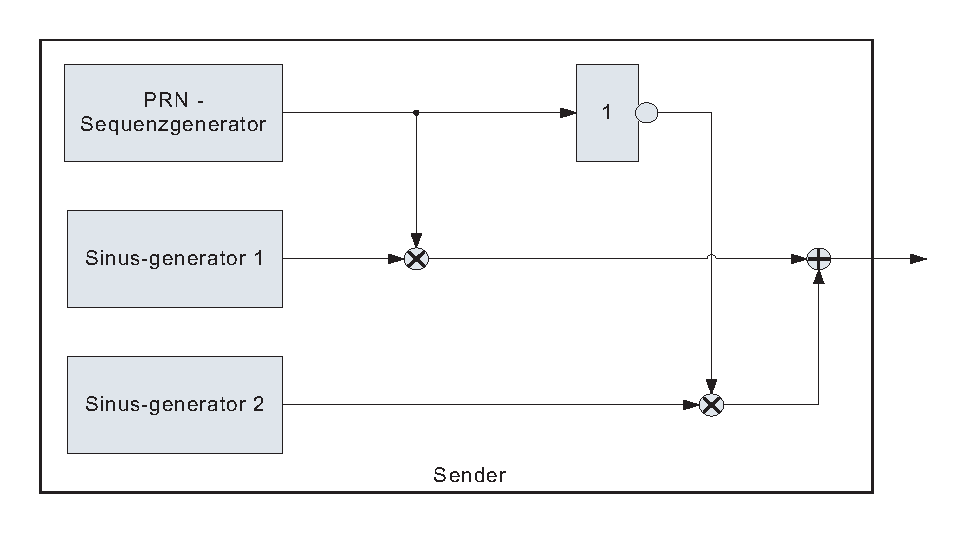
\includegraphics[width=10cm]{bilder/sender/sender_blockschaltbild}
	\caption{Sender Blockschaltbild}
	\label{abb:sender_blockschaltbild}\index{Sender Blockschaltbild}
\end{figure}

Mittels des in Abb. \ref{abb:sender_blockschaltbild} dargestellten Systems werden wir die zu �bertragenden Signale erzeugen. Es besteht in erster Linie aus einem Pseudo-Zufallszahlen-Generator, dessen Ausgangssignal mit Hilfe eines einfachen FSK-Modulators moduliert werden soll. Eine detailliertere Beschreibung der einzelnen Komponenten wird in den folgenden Kapiteln erarbeitet.